\chapter{Non-Markovian Reinforcement Learning}

\section{Non-Markovian goals}

\label{sec:non-markov}

The goal of a RL agent is to maximize the cumulative rewards received.  A
goal, or a task, is said \emph{non-Markovian} if the rewards do not satisfy
the Markov assumption on rewards, i.e:
\begin{equation}
	r_{t+1} \not\perp s_i, a_i, r_i \given s_t, a_t
	\qquad \text{for some $t, i$, with $0 \le i < t$}
	\label{eq:markov-rewards}
\end{equation}
Of course, this can happen only if the environment cannot be modelled with an
MDP. Excellent algorithms exists for MDPs; instead, non-Markovian goals are
much more difficult to learn.  There are two main causes for non-Markovian
rewards: partial observations and temporally-extended tasks. We'll thoroughly
analyze both scenarios.


\subsection{Partial observations}

\label{sec:partial-obs}

Up to this point, we didn't need to distinguish between observations and
states. In fact, we assumed that the agent can directly observe the
environment states and act accordingly (we defined the policy as a function of
the state). Unfortunately, this is often not the case: we only get to see
something that depends on the current state, but it's not. These systems can
be modelled with a \emph{Partially Observable Markov Decision Process}
(POMDP)\nomenclature{POMDP}{Partially Observable Markov Decision Process}.
POMDPs are a generalization of MDPs for partial observations. From now on, we
will denote with $\stateS$ the environment state space and with $\obsS$ the
observation space. Formally, a discrete-time POMDP is a 7-tuple ${\langle
\stateS, A, T, R, \obsS, O, \discount \rangle}$, where $\stateS, A, T, R$ are
defined as in MDPs, $\obsS$ is the observation space, and $O$ is the
observation function ${O: S \to \obsS}$.

The graphical model of a POMDP is shown in Figure~\ref{fig:pomdp}.
\begin{figure}

	\centering
	\begin{tikzpicture}
		\matrix [
			column sep={1.5cm,between origins}, row sep={1cm,between origins},
		] {
			\node (om1) [observed node, label=above:$o_{t-1}$] {}; \&
			\node (am1) [observed node, label=above:$a_{t-1}$] {}; \&
			\node (o) [observed node, label=above:$o_{t}$] {}; \&
			\node (a) [observed node, label=above:$a_{t}$] {}; \\
			\node (stm1) [node, label=below left:$s_{t-1}$] {};
			\& \&
			\node (st) [node, label=below left:$s_{t}$] {}; \& \&
			\node (st1) [node, label=below left:$s_{t+1}$] {}; \\
			\& \&
			\node (r) [observed node, label=below:$r_{t}$] {}; \& \&
			\node (r1) [observed node, label=below:$r_{t+1}$] {}; \\
		};
		\draw [->] (stm1) -- (om1);
		\draw [->] (st) -- (o);
		%
		\draw [->] (st) -- (r);
		\draw [->] (st1) -- (r1);
		%
		\draw [->, dotted] (om1) -- node [midway] {?} (am1);
		\draw [->, dotted] (o) -- node [midway] {?} (a);
		%
		\draw (st) edge [<-] (stm1) edge [<-] (am1);
		\draw (st1) edge [<-] (st) edge [<-] (a);

		\draw [dashed, gray] (st1) -- +(0.8,0);
		\draw [dashed, gray] (stm1) -- +(-0.8,0);
	\end{tikzpicture}
	\caption{The Directed Graphical Model of a POMDP. White nodes are
	unobservable. For simplicity, the rewards in this graph depend just on the
	current state $s_t$, not on transitions ${(s_t, a_t, s_{t+1})}$.}
	\label{fig:pomdp}
\end{figure}
The sequence of states ${\langle s_0, s_1, \dots \rangle}$, which is the
environment dynamics, still satisfies the Markov assumption (it forms a Markov
chain). In a POMDP, this dynamics exists but is unobservable. What we can
see, instead, is a sequence of observations ${ \langle o_0, o_1, \dots
\rangle}$. Each of them is generated from the corresponding state, through the
(possibly nondeterministic) observation function. Actions and policies can
only act in response to observations, not states.

The dotted arrows in Figure~\ref{fig:pomdp} have a question mark on them,
because that dependency is our choice. As designers, we're free to select the
informations that the agent should take into account when selecting an action.
Is the last observation enough to decide? Or, more precisely, among all
possible policies, do POMDPs always admit an optimal policy of the form
$\optimal\policy: \obsS \to A$? Unfortunately, the answer is no. Other
informations are needed.

When the POMDP transition and observation functions are known, a common
solution is to estimate the current unobservable state and decide the action
from this belief. With deterministic functions, the agent can iteratively
restrict the set of possible states by eliminating those inconsistent with the
observations received. More commonly, these functions are nondeterministic,
and the estimation algorithm is some recurrent probabilistic inference.
In both cases, the algorithm would produce a belief of the current state,
denoted with $b(s_t)$. We can represent the general procedure, at any
instant~$t$, with the following computation:
\begin{center}
	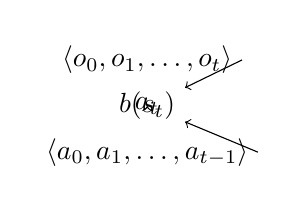
\begin{tikzpicture}
		\matrix [column sep=2em] {
			\node (o) {$\langle o_0, o_1, \dots, o_t \rangle$}; \\
			\&
			\node (s) {$b(s_t)$}; \& \node (an) {$a_t$}; \\
			\node (a) {$\langle a_0, a_1, \dots, a_{t-1} \rangle$}; \\
		};
		\draw [->] (o.east) -- (s);
		\draw [->] (a.east) -- (s);
		\draw [->] (s) -- (an);
	\end{tikzpicture}
\end{center}
Since these beliefs depend on the whole sequence of observations, computing
the next action from $b(s_t)$ also makes it dependent from the whole history.

Standard RL algorithms cannot be applied to POMDPs, because the state space is
not observable. Also, since we allow the transition and observation functions
to be unknown, no estimation could be carried out anyway.  There is a clear
difference between MDPs and POMDPs. Still, RL algorithms are frequently
applied to POMDPs. Not surprisingly, they perform very poorly on these
environments. This is a subtle mistake, because determining whether we're
observing the state space is the same as answering the following question:
does the observation space capture the ``relevant'' dynamics of the system?
Or, more precisely, does an equivalent MDP $\langle \obsS, A, T_\obsS,
R_\obsS, \discount' \rangle$, that produces the same rewards, exist?  If both
functions $T_\obsS: \obsS \times A \times \obsS \to \R$ and $R_\obsS: \obsS
\times A \times \obsS \to \R$ exist and produce the same rewards, the
environment can be successfully modelled and solved as an MDP.
However, since this is often not the case, we cannot apply RL algorithms to
POMDPs. Figure~\ref{fig:pomdp-as-mpd} represents this situation.

\begin{figure}
	\centering
	\begin{tikzpicture}[
			hidden arc/.style={->, densely dotted},
			box/.style={rounded corners=5pt, inner sep=1.8ex, draw=#1!50,
				fill=#1!20},
		]
		\matrix [
			column sep={1.6cm,between origins}, row sep={1.3cm,between origins},
		] {
			\node (stm1) [node, label=above:$s_{t-1}$] {}; \& \&
			\node (st) [node, label=above:$s_{t}$] {}; \& \&
			\node (st1) [node, label=above:$s_{t+1}$] {}; \\
			\&
			\node (am1) [observed node, label=above:$a_{t-1}$] {}; \&
			\node (r) [observed node, label=left:$r_{t}$] {}; \&
			\node (a) [observed node, label=above:$a_{t}$] {}; \&
			\node (r1) [observed node, label=left:$r_{t+1}$] {}; \\
			\node (om1) [observed node, label=below:$o_{t-1}$] {}; \& \&
			\node (o) [observed node, label=below:$o_{t}$] {}; \& \&
			\node (o1) [observed node, label=below:$o_{t+1}$] {}; \\
		};
		\draw [hidden arc, bend left] (stm1) to (om1);
		\draw [hidden arc, bend left] (st) to (o);
		\draw [hidden arc, bend left] (st1) to (o1);
		%
		\draw [hidden arc] (st) -- (r);
		\draw [hidden arc] (st1) -- (r1);
		%
		\draw [hidden arc] (stm1) -- (st);
		\draw [hidden arc] (st) -- (st1);
		\draw [hidden arc] (am1) -- (st);
		\draw [hidden arc] (a) -- (st1);
		%
		\draw [dashed, gray] (st1) -- +(0.8,0);
		\draw [dashed, gray] (stm1) -- +(-0.8,0);
		%
		\draw [->] (o) -- (r);
		\draw [->] (o1) -- (r1);
		%
		\draw [->] (om1) -- (o);
		\draw [->] (o) -- (o1);
		\draw [->] (am1) -- (o);
		\draw [->] (a) -- (o1);
		%
		\draw [dashed, gray] (st1) -- +(0.8,0);
		\draw [dashed, gray] (stm1) -- +(-0.8,0);
		\draw [dashed, gray] (o1) -- +(0.8,0);
		\draw [dashed, gray] (om1) -- +(-0.8,0);
		% boxes
		\begin{pgfonlayer}{below}
			\path coordinate (st-up) at ($(st)+(0,1em)$);
			\node [fit={(stm1) (st1) (st-up)}, box=gray,
				pin=right:{\footnotesize hidden dynamics}
			] {};
			\node [fit={(om1) (o1) ($(a.north)+(0,1ex)$) ($(o.south)+(0,-1ex)$)},
				box=orange, pin=right:{\footnotesize MDP assumption}] {};
		\end{pgfonlayer}
	\end{tikzpicture}
	\caption{The dotted arrows \protect\tikz [baseline=-0.5ex] \protect\draw
	[densely dotted, ->] (0,0) to +(1.5em,0); represent the dependencies in a
	POMDP model. Solid arrows \protect\tikz [baseline=-0.5ex] \protect\draw
	[->] (0,0) to +(1.5em,0); show the MDP assumption over the same observable.
	This is usually a very poor approximation of the real dynamics.  }
	\label{fig:pomdp-as-mpd}
\end{figure}

\begin{example}
	As we've seen from Example~\vref{ex:board-games}, the game of Chess can
	be modelled with an MDP if we consider as states the vectors of positions of
	all pieces on the board. Let's suppose, instead, the observations available
	are images of the board after each move (if the pieces can be distinguished,
	these could even come from a real play). Each image completely captures the
	state of the game because, for each move of the agent and the opponent,
	we're able to accurately predict the image that will follow. This is a
	transition $T_\obsS$ over images. Similarly, a reward function $R_\obsS$ can
	simply return $+1$ or $-1$ for images with checkmates and 0 otherwise. These
	functions can be unknown and don't need to be defined.

	Suppose, instead, that the agent can only observe the left-hand side of the
	board (columns a-d, for example). In this case, each image provides an
	incomplete view over the state of the game. In fact, in order to determine
	the best action we must consider whether there are some attacking pieces on
	the hidden region. In this case, classic RL algorithms would perform poorly,
	because without any memory about the position of the hidden pieces, 
	it's not possible to predict the next image and reward from the current
	observation.
	\label{ex:chess-partial-obs}
\end{example}

\begin{example}
	Let's consider a classic control problem: the swing-up of an inverted
	pendulum. A pendulum can freely rotate by 360° around a hinge. The agent, at
	each discrete time step, can apply torques to this active joint.  The goal
	is to stabilize the pendulum in the upward position, which is the
	configuration of unstable equilibrium. In order to solve this problem with
	Reinforcement Learning, we need to define the spaces $S$ and $A$ of the MDP.
	In this domain, actions are continuous torques, which may be represented in
	a normalized range: $A \coloneqq [-1, +1] \subseteq \R$. The angle of the
	pendulum $\theta$ with respect to some fixed reference completely determines
	the position of the masses. Is the reward Markovian with respect to $S
	\coloneqq \{\theta \in [-\pi, +\pi]\}$? No, because the agent is rewarded
	when the pendulum \emph{stops} in the upward position. So, the appropriate
	state space consists of both $\theta$ and $\dot\theta$.

	Including the momentum in the state space is very common for mechanical
	systems. However, this can be also necessary for games. In fact, just
	looking at a single frame, the agent has no clue about how all the elements
	in the picture are moving.  For example, in a video game where the agent has
	to hit a moving ball, the optimal policy certainly needs to observe also its
	direction.
	\label{ex:motion}
\end{example}


\subsection{Temporally-extended goals}

\label{sec:tempoal-goals}

The previous section has shown how partial observations may falsify the Markov
assumption on rewards. A second possibility is to have a complete observation
of the state ($\obsS = \stateS$) but a task that is intrinsically
non-Markovian. This is the case when each reward is computed from the whole
history of events
\begin{equation}
	r_t = R(\langle s_0, s_1, \dots, s_t \rangle) \qquad \forall t \in \Z
	\label{eq:nm-rewards}
\end{equation}
with $R: \stateS^* \to \R$. The sequence of states $\trace
\coloneqq \langle s_0, s_1, \dots, s_t \rangle$ will be also called
execution \emph{trace}. In general, with the term ``trace'' we indicate any
sequence that is produced during a run. We adopt a similar notation to those
we've seen for interpretations of temporal logics.

Goals defined by rewards of equation~\eqref{eq:nm-rewards} are said
``temporally-extended'' because they take into account multiple timesteps. Why
should we define a reward function that is explicitly non-Markovian? One
possibility is that we want our agent to drive the environment through a
\emph{sequence} of states, instead of just reaching a single configuration.
However, as we will see, we don't need to restrict to sequences, because we
may define very complex reward functions.

\begin{example}
	Let's suppose the agent can control a light bulb through a switch, and we
	want the light to be set on, then off again. The agent will be rewarded if,
	at the end of the episode, the light has been set on only once.  The
	environment is extremely simple: its state may be completely described by a
	Boolean variable, ``lightOn'', which reflects the status of the light.
	Still, in order to valuate whether the task has been accomplished, it's not
	sufficient to check whether the light is off at the end of the episode; we
	also need to ensure that, \emph{during the whole episode}, it has been
	switched on only once.
	\label{ex:light}
\end{example}

We now define a model that, by generalizing MDPs, can describe this large
class of problems.
\begin{definition}
	A \emph{Non-Markovian Reward Decision Process}
	(NMRDP)\nomenclature{NMRDP}{Non-Markovian Reward Decision
	Process}~\cite{bib:nmrdp-logic-first} is a tuple $\langle \stateS, A, T, R,
	\discount \rangle$, where $\stateS, A, T, \discount$ are defined as for
	MDPs, and $R: \stateS^* \to \R$ is a non-Markovian reward function, which
	computes the reward at time $t$ as $r_t = R(\langle s_0, s_1, \dots, s_t
	\rangle)$.
\end{definition}

Every NMRDP admits an optimal policy as ${\optimal\policy: S^* \to A}$, which
computes actions from the history of states. So, we'll only consider policies
with this form. In order to define optimality, we would need to proceed as for
MDPs, by defining value functions. However, this is sightly more complex,
since as a consequence of non-Markovian rewards, value functions can
only predict the future expected discounted return, if the past history is
given. They effectively compare policies on traces, rather than single
states. The simplest case is the valuation of any initial state, whose value
function is~\cite{bib:nmrdp-logic-first}:
\begin{equation}
	v_{\policy}(\langle s_0 \rangle) \coloneqq \E_{\policy} \Biggl[\,
		\sum_{t=0}^{T} \discount^t R(\langle s_0, s_1, \dots, s_t \rangle)
		\,\Biggr]
\end{equation}
Informally, an NMRDP policy~$\optimal\policy$ is optimal if it maximizes the
value function of future states. However, we won't further delve into the
definition of optimality and value functions, because common solution methods
(that we'll see in Section~\ref{sec:nmrdp-solution}) transform NMRDPs into
standard MDPs, that we already know how to solve.


\subsubsection*{NMRDP with \ldl{} rewards}

Non-Markovian reward functions have huge domains. Defining them by listing all
the traces that should be (positively or negatively) rewarded is unfeasible,
even for the simplest cases. Fortunately, as we already know from
Chapter~\ref{ch:logics}, temporal logics are powerful formalisms that allow to
concisely define groups of traces. So, a very effective way to declare
non-Markovian rewards is through a set of pairs $\set{(\formula_i,
r_i)_{i=1}^m}$, where each $\formula_i$ is a \ldl{} formula and $r_i$ is its
associated reward~\cite{bib:degiacomo-logic-nmrdp}. The reward $r_i$ will be
produced whenever a trace satisfies~$\formula_i$. So, the reward function is
defined as:
\begin{equation}
	R(\trace) \coloneqq \sum_{i \,:\, \trace \models \formula_i} r_i
	\label{eq:ldlf-rewards}
\end{equation}
It follows that an equivalent way to define NMRDPs is: $\langle S, A, T,
\set{(\formula_i, r_i)_{i=1}^m}, \discount \rangle$.

In this thesis, rewards will be always declared with \ldl{} formulae. However,
the same discussion also applies to \ltl{}. Also, we may have noticed that the
adoption of temporal logics requires a state space that is composed of
propositional interpretations. This will be addressed in Section~\ref{sec:rb}.


\section[Reinforcement Learning with LDLf specifications]%
{Reinforcement Learning with \ldl{} specifications}

\label{sec:non-markov-solutions}

This section illustrates how to learn optimal policies for a large class of
problems among those introduced in Section~\ref{sec:non-markov}. The main idea
behind the techniques presented here is to formulate an appropriate NMRDPs
with \ldl{} rewards, and to solve it through an equivalent Markov Decision
Process. Since many learning algorithms exist for MDPs, this translation can
be considered as a solution for the original problem.


\subsection[RL for NMRDPs with LDLf rewards]%
{RL for NMRDPs with \ldl{} rewards}

\label{sec:nmrdp-solution}

\subsubsection*{RL for NMRDPs}

Before looking at the construction, we need to define what is an
\emph{equivalent} MDP and what are its properties.

% General equivalence
\begin{definition}
	\cite{bib:nmrdp-logic-first} An NMRDP $\nmrdpS \coloneqq \langle S, A, T, R,
	\discount \rangle$ is \emph{equivalent} to an extended MDP $\mdpS \coloneqq
	\langle S', A, T', R', \discount \rangle$ if there exist two functions
	$\tau: S' \to S$ and $\sigma: S \to S'$ such that:
	\begin{enumerate}
		\item $\forall s \in S : \tau(\sigma(s)) = s$;
		\item $\forall s_1, s_2 \in S$ and $s_1' \in S'$: if $T(s_1, a, s_2) > 0$
			and $\tau(s_1') = s_1$, there exists a unique $s_2' \in S'$ such that
			$\tau(s_2') = s_2$ and $T'(s_1', a, s_2') = T(s_1, a, s_2)$.
		\item For any feasible trajectory $\langle s_0, a_1, \dots, s_{n-1}, a_n
			\rangle$ of $\nmrdpS$ and $\langle s_0', a_1, \dots, s_{n-1}', a_n
			\rangle$ of $\mdpS$, such that $\tau(s_i') = s_i$ and $\sigma(s_0) =
			s_0'$, we have $R(\langle s_0, a_1, \dots, s_{n-1}, a_n
			\rangle) = R'(\langle s_0', a_1, \dots, s_{n-1}', a_n \rangle)$.
	\end{enumerate}
	\label{def:nmrdp-mdp-equiv}
\end{definition}
Conditions 1 and 2 require that every feasible trajectory of the NMRDP can be
simulated with a trajectory of the MDP. Condition 3 forces corresponding
trajectories to produce the same rewards. So, the equivalent MDP completely
captures the dynamics of the NMRDP. As we will see, in order to do this, the
new state space $S'$ needs to include the old states $S$ and some
history-related informations. Since $S'$ is always larger than $S$, the
equivalent MDP is also called ``extended''.

\begin{definition}
	\cite{bib:nmrdp-logic-first} Let $\policy': S' \to A$ be a policy for the
	MDP $\mdpS$. The corresponding policy $\policy: S^* \to A$ of the NMRDP
	$\nmrdpS$ is defined as $\policy(\langle s_0, \dots, s_n \rangle) \coloneqq
	\policy'(s_n')$ where $\langle s_0', \dots, s_n' \rangle$ is the
	corresponding trajectory for $\langle s_0, \dots, s_n \rangle$.
\end{definition}
As we can see $\policy'$, is a stationary policy. A very important result that
allows to correlate the solutions between the two classes of problems is the
following:
\begin{theorem}
	\cite{bib:nmrdp-logic-first} For any policy $\policy'$ for the MDP $\mdpS$,
	its corresponding policy $\policy$ for the NMRDP $\nmrdpS$, and $s \in S$,
	we have $v_\policy(s) = v_{\policy'}(\sigma(s)).~$\footnote{In this equation,
	$v$ refers to the value function for NMRDPs and MDPs respectively.}
\end{theorem}
As a corollary of the previous theorem, any optimal policy of the MDP has a
corresponding policy that is optimal for the NMRDP. This is is the result we
were looking for: by applying classic RL algorithms, we can learn optimal
policies of MDPs that apply to their equivalent NMRDP. In practice, we don't
need to translate the policy $\policy'$ to the non-stationary
equivalent~$\policy$.  It is possible to apply the trained RL agent directly
to the NMRDP, by continuously transforming each observation $s$ through the
translation function~$\sigma: S \to S'$.


\subsubsection*{\ldl{} rewards}

We will now define a specific MDP expansion for NMRDPs with \ldl{} rewards.
In fact, if the rewards are specified through \ldl{} or \ltl{}, it is possible
to create extended MDPs that are very compact. We recall that a NMRDP with
\ldl{} rewards is a tuple $\nmrdpS \coloneqq {\langle S, A, T,
\set{(\formula_i, r_i)_{i=1}^m}, \discount \rangle}$, where $S \coloneqq
2^\fluents$ is a set of propositional interpretations and $\formula_i$ are
\ldl{} formulae on the set of fluents~$\fluents$.

First, using the methods presented in Section~\ref{sec:ldlf-to-automa}, we
transform each reward formula~$\formula_i$ to its associated minimal
DFA,~${\automa_i \coloneqq \langle 2^\fluents, Q_i, q_{i0}, \delta_i, F_i
\rangle}$. Then, we state the following:
\begin{definition}
	\cite{bib:degiacomo-logic-nmrdp} Given an NMRDP with \ldl{} rewards~$\nmrdpS
	= \langle S, A, T, \set{(\formula_i, r_i)_{i=1}^m},\allowbreak \discount
	\rangle$, we define the equivalent extended MDP~$\mdpS \coloneqq {\langle
	S', A', T', R', \discount \rangle}$, where:
	\begin{itemize}
		\item $S' \coloneqq Q_1 \times \dots \times Q_m \times S$ is the set of
			states
		\item $A' \coloneqq A$
		\item $T' : S' \times A' \times S' \to [0, 1]$ is defined as:
			\[
				T'((q_1, \dots, q_m, s), a, (q_1', \dots, q_m', s')) \coloneqq
				\begin{cases}
					T(s, a, s') & \text{if $\forall i : \delta_i(q_i, s') = q_i'$} \\
					0 & \text{otherwise}
				\end{cases}
			\]
		\item $R' : S' \to \R$ is defined as\footnote{There is a slight difference
			with the original definition in~\cite{bib:degiacomo-logic-nmrdp}, which
			accounts for a small notation difference in some previous definitions:
			$R(s_t)$ is assumed to produce $r_t$, not $r_{t+1}$.}:
			\[
				R((q_1, \dots, q_m, s)) \coloneqq \sum_{i\, :\, q_i \in F_i} r_i
			\]
	\end{itemize}
	\label{def:ldlf-eq-mdp}
\end{definition}
As we can see from this definition, the extended MDP augments the original
model with all the automata~$\automa_i$ corresponding to the $m$ temporal
goals. After each observation, both the original system and every
component~$\automa_i$ are advanced accordingly, in parallel. The reward
function, which is now Markovian, can produce the same rewards as in the
original formulation (see equation~\eqref{eq:ldlf-rewards}) because all the
necessary information has been included in the state space.

\begin{theorem}
	\cite{bib:degiacomo-logic-nmrdp} The NMRDP with \ldl{} rewards $\nmrdpS =
	{\langle S, A, T, \set{(\formula_i, r_i)_{i=1}^m}, \discount \rangle}$ is
	equivalent to the MDP $\mdpS$ of Definition~\ref{def:ldlf-eq-mdp}.
\end{theorem}
The last theorem states that our construction creates an equivalent MDP,
according to the Definition~\ref{def:nmrdp-mdp-equiv}. Any NMRDP can be
formulated as an MDP, if enough history is included in the state space. So,
what is really interesting about this translation is that the expanded MDP has
a minimal state space. This is possible because the current state of the
automaton~$\automa_i$ is a sufficient information that retains just enough
history to render the rewards $r_i$ Markovian. We have:
\begin{theorem}
	\cite{bib:degiacomo-logic-nmrdp} If every automaton $\automa_i \,(1 \le i
	\le m)$ is minimal, then the extended MDP of
	Definition~\ref{def:ldlf-eq-mdp} is minimal.
\end{theorem}

To recap, in this section, we've shown how to train an agent on a
Non-Markovian Reward Decision Process, by applying classic RL algorithms on
the equivalent MDP. Once the relevant fluents have been selected, we need to
express our goal as \ldl{} conditions that are associated to a positive reward
(or, maybe, conditions for negative rewards). We will see some practical
examples in the following section, where we study how to deal with multiple
representations of the same configuration of the environment. 


\subsection[RL with LDLf restraining specifications]%
{RL with \ldl{} restraining specifications}

\label{sec:rb}

\subsubsection{Multiple representations}

The solution for NMRDPs that we've seen in the previous section is elegant and
effective. However, at first sight, it may only seem applicable in very simple
state spaces, that are composed of Boolean valuations for sets of fluents
(for example, at some time $t$, we might have a state $s_t$ in which:
$\set{\text{\texttt{HaveKey}} = \const{True}, \text{\texttt{DoorClosed} =
\const{False}}}$). This is not true, because we must remember that the NMRDP
is just a model that we've defined. We're free to adopt a new formalism, where
the sequence of observations produced by the environment is decoupled from the
trace where our formulae are interpreted on. The ideas presented here have
been developed in~\cite{bib:bolt}.

Let's denote with $W$ the set of world states. This is an abstract
representation of the environment configuration that is inaccessible to the
agent. Instead, it receives observations that directly depend on these states.
We can represent this sensory input with a function $f_S: W \to S$.
Frequently, $S$ is a multidimensional space, so the observations $s \in S$ are
also called \emph{features vectors}, or simply \emph{features}. Assuming that
these features are the state space of a Markov Decision Process, we can apply
RL on~$S$.

We now assume that there is a second function $f_\highlevelS: W \to
\highlevelS$, with $\highlevelS \coloneqq 2^\fluents$, that given a world
state, assigns a truth value to all fluents in~$\fluents$.  This creates two
representations with different roles: $S$ is a \emph{low-level} features space
that can be complex, noisy and difficult to interpret directly; $\highlevelS$
is a \emph{high-level} logic representation of the same world states. To any
configuration $w \in W$ corresponds a pair of the representations $s \in S$
and $l \in \highlevelS$. See Figure~\ref{fig:representations}.

\begin{figure}
	\centering
	\begin{tikzpicture}[
			every node/.append style={font=\small},
		]
		\matrix [
			column sep={2cm,between origins}, row sep={1.2cm,between origins},
		] {
			\coordinate (ltrace); \&
			\node (ltm1) [observed node, label=above:$l_{t-1}$] {}; \&
			\node (lt) [observed node, label=above:$l_t$] {}; \&
			\node (lt1) [observed node, label=above:$l_{t+1}$] {}; \\
			\&
			\node (wtm1) [node, label=above right:$w_{t-1}$] {}; \&
			\node (wt) [node, label=above right:$w_t$] {}; \&
			\node (wt1) [node, label=above right:$w_{t+1}$] {}; \\
			\coordinate (strace); \&
			\node (stm1) [observed node, label=below:$s_{t-1}$] {}; \&
			\node (st) [observed node, label=below:$s_t$] {}; \&
			\node (st1) [observed node, label=below:$s_{t+1}$] {}; \\
		};
		\draw [->] (wtm1) -- (wt);
		\draw [->] (wt) -- (wt1);
		\path [->] (wtm1) edge (ltm1) edge (stm1);
		\path [->] (wt) edge (lt) edge (st);
		\path [->] (wt1) edge (lt1) edge (st1);
		%
		\node (high-text) [anchor=east, xshift=0.7cm] at (ltrace) 
			{high-level $l_i \in \highlevelS = 2^\fluents$};
		\node (low-text) [anchor=east, xshift=0.7cm] at (strace)
			{low-level $s_i \in S$};
		%\begin{pgfonlayer}{below}
		%	\node [fit={(high-text) (lt1)}, box=blue!50!gray, inner sep=9pt] {};
		%	\node [fit={(low-text) (st1)}, box=orange, inner sep=9pt] {};
		%\end{pgfonlayer}
		\draw [->, dotted] (ltm1) -- (lt) -- (lt1) -- +(2cm,0)
			node [right, black] {trace $\trace$};
		%
		\draw [<-, darkgray, dashed] (wtm1) -- +(-1, 0);
		\draw [->, darkgray, dashed] (wt1) -- +(1, 0);
	\end{tikzpicture}
	\caption{Every world state generates both high-level and low-level
		configurations.}
	\label{fig:representations}
\end{figure}

This distinction is powerful: it allows us to declare temporally-extended
goals with \ldl{} on the set of fluents~$\fluents$, while the agent receives
and works with a different set of features. We now formally define a specific
problem that is possible thanks to this distinction.


\subsubsection{Restraining Specifications}

Consider a Reinforcement Learning agent on the MDP $\mdpS \coloneqq \langle
S, A, T, R \rangle$\footnote{
	The discount factor has been omitted in this section, because it doesn't
	apply to the problems we study here. So, it may be simply regarded as
	tunable parameter.
}.
This already defines the environment dynamics and the agent's optimal policy.
We now want to modify the agent's behaviour by declaring an additional
temporally-extended goal on some fluents~$\fluents$.  The purpose is to train
an agent that pursues the original rewards, while complying with the
additional specification we provided.  As we know from
Section~\ref{sec:tempoal-goals}, the \ldl{} goals are just a clever way of
declaring a non-Markovian reward function. These will be summed with the
original rewards, so that the agent will try to pursue both\footnote{
	The agent can behave optimally with respect to this combination, but this
	doesn't necessarily mean that this is the policy we were looking for.
	Finding the appropriate combination of rewards is a general issue in RL.
}.
We call this additional module, which reads the current fluents' configuration
and sends the non-Markovian reward back, as the ``Restraining
Bolt''~\cite{bib:bolt}. This term, borrowed from Science Fiction, suggests
that with this additional construction, we're able to modify the ``natural''
agent's behaviour. In this context, the \ldl{} goals $\set{(\formula_i,
r_i')_{i=1}^m}$ are referred to as ``restraining specifications''. The general
setup is presented in Figure~\ref{fig:rb-schema}.
\begin{figure}
	\centering
	\begin{tikzpicture}[
			every node/.append style={font=\scriptsize},
			arrow/.style={->, semithick},
		]
		\node (rb-features) [block] {RB\\features\\extractor};
		\node (rb) [block, right=of rb-features]  {Restraining\\Bolt};
		\node (agent) [block, right=of rb.south east, anchor=south west,
				minimum width=3cm, minimum height=3cm]
			{Learning agent};
		\node (agent-south) [below=1.2cm of agent.south east, inner sep=0pt] {};
		\node (rb-features-south) [below=1.2cm of rb-features.south west, inner sep=0pt] {};
		\node (world-block) [block, fit=(rb-features-south) (agent-south),
			inner sep=0, minimum height=1cm] {};
		\node at (world-block.center) {\scriptsize World};
		\node (agent-features) [block, above=0.5cm of rb-features]
			{LA\\features\\extractor};
		%
		\draw [arrow] (agent.east) -- +(0.7,0) |-
			node [right, pos=0.2] {$a$} (world-block);
		\coordinate (world-west) at ($(world-block.west)+(-0.7,0)$);
		\node [anchor=east] at (world-west |- rb-features.west) {$w$};
		\draw [arrow] (world-block.west) -- (world-west) |- (rb-features);
		\draw [arrow] (world-west |- rb-features.west) |- (agent-features);
		\draw [arrow] (rb-features) -- node [above] {$l$} (rb);
		\draw [arrow] (rb) -- node [above] {$r'$} (agent.west |- rb.east);
		\draw [arrow] (agent-features) -- node [above] {$s$}
			(agent.west |- agent-features);
		\draw [arrow] (rb.north) -- +(0,0.5) -- node [above] {$\vec{q}$} 
			($(rb.north -| agent.west)+(0,0.5)$);
		\draw [arrow] (world-block.north -| agent.south) --
			node [left] {$r$} (agent.south);
	\end{tikzpicture}
	\caption{Learning agent with Restraining Bolt applied. $r$ is the classic
	MDP reward; $r'$ is the additional non-Markovian reward generated.}
	\label{fig:rb-schema}
\end{figure}
Notice, in particular, that the learning agent has access to the original
observations~$s$ and rewards~$r$, and the additional non-Markovian
rewards~$r'$.  The quantity $\vec{q}$ will be discussed shortly. Let's now
formalize this problem.
\begin{definition}
	\cite{bib:bolt} A \emph{RL problem with \ldl{} restraining specifications}
	is a pair $\langle \mdpS, \const{RB} \rangle$, where: $\mdpS \coloneqq
	\langle S, A, T, R \rangle$ represents a learning agent, and $\const{RB}
	\coloneqq \langle \highlevelS, \set{(\formula_i, r_i')_{i=1}^m} \rangle$ is
	a Restraining Bolt formed by a set of \ldl{} formulae $\formula_i$ over
	$\fluents$ with associated rewards~$r_i'$.
	\label{def:rb-problem}
\end{definition}

We can't simply apply a RL algorithm on the rewards $r_i, r_i'$ over the state
space~$S$, because $r_i'$ are non-Markovian in $S$. What we can do, instead,
is to formulate a NMRDP with \ldl{} rewards, that we already know how to
solve. The complete proof is shown in~\cite{bib:bolt}
and~\cite{bib:favorito-thesis}.	What we see here is a shorter explanation that
just highlights the main concepts.

We first observe that, in Definition~\ref{def:rb-problem}, the MDP and the
Restraining Bolt are completely distinct; their only interaction is in the sum
of the rewards they produce (let's denote with $\bar{r}_i \coloneqq r_i +
r_i'$ the combined reward). So, to simplify the computation, we may keep
these two problems separate, transform the restraining specifications to their
equivalent MDP and combine them later. This is possible because, given two
MDPs, $\mdpS_a = \langle S_a, A, T_a, R_a \rangle$ and $\mdpS_b = \langle S_b,
A, T_b, R_b \rangle$, the following~$\mdpS_{ab} \coloneqq \langle S_{ab}, A,
T_{ab}, R_{ab} \rangle$, with states $S_{ab} \coloneqq S_a \times S_b$,
transition function $T_{ab}: S_{ab} \times A \times S_{ab} \to \R$ and rewards
\[
	R_{ab}((s_a, s_b), a, (s_a', s_b')) \coloneqq R_a(s_{a}, a, s_{a}') +
	R_b(s_{b}, a, s_{b}')
\]
is still an MDP.  Note that we didn't define $T_{ab}$. This is not required,
as in RL, it is sufficient that this unknown function exists; and by the laws
of probability, this is certainly the case, because the existence of $T_a$ and
$T_b$ is a stronger requirement.

Every Restraining Bolt $\const{RB} = \langle \highlevelS, \set{(\formula_i,
r_i')_{i=1}^m} \rangle$ defines a NMRDP with \ldl{} rewards
$\nmrdpS_{\const{RB}} \coloneqq \langle \highlevelS, A, T_\highlevelS,
\set{(\formula_i, r_i')_{i=1}^m} \rangle$, with states $\highlevelS =
2^\fluents$ and $T_\highlevelS$ as the unknown transition function over
fluents configurations. This is a problem that we already know how to solve.
By directly applying Definition~\ref{def:ldlf-eq-mdp}, we can write the
extended MDP~$\mdpS_{\const{RB}} \coloneqq \langle S_{\const{rb}}, A,
T_{\const{rb}}, R_{\const{rb}} \rangle$ that is equivalent to the
NMRDP~$\nmrdpS_{\const{RB}}$. Notice in particular, that the state space
becomes: $S_{\const{rb}} \coloneqq Q_1 \times \dots \times Q_m \times
\highlevelS$, where each $Q_i$ is the set of states of the $i$-th automaton.
For brevity, we will denote elements of $Q_1 \times \dots \times Q_m$ with
$\vec{q}$, because they are vectors of automaton states.

We can now combine the original MDP~$\mdpS$ with the one generated from the
Restraining Bolt~$\mdpS_{\const{RB}}$, just like we've done for $\mdpS_{ab}$,
to obtain a new unified MDP that is defined as $\mdpS' \coloneqq \langle S',
A, T', R' \rangle$, where:
\begin{itemize}
	\item $S' \coloneqq Q_1 \times \dots \times Q_m \times \highlevelS \times S$
	\item $T' : S' \times A \times S' \to \R$ with:
		\begin{multline*}
			T'((q_1, \dots, q_m, l, s), a, (q_1', \dots, q_m', l', s')) \coloneqq \\
			\begin{cases}
				T_{l,s}((l,s), a, (l',s')) &
					\text{if $\forall i : \delta_i(q_i, l') = q_i'$} \\
				0 & \text{otherwise}
			\end{cases}
		\end{multline*}
	\item $R' : S' \times A \times S' \to \R$ with:
		\[
			R'((q_1, \dots, q_m, l, s), a, (q_1', \dots, q_m', l', s')) \coloneqq
			\sum_{i\, :\, q_i' \in F_i} r_i' + R(s, a, s')
		\]
\end{itemize}
Both $T_{l,s}$, that is the joint transition function of the symbols $s$ and
$l$, and the original reward function, $R$, are unknown: we only observe the
samples produced while the agent plays. Instead, we have to move all
automata and return the associated rewards, because this is a dynamics we've
defined.

To this point, we've reduced the original problem of
Definition~\ref{def:rb-problem} to standard RL on the MDP~$\mdpS'$. However,
we can move one step further. In fact, the combined rewards $\bar{r}_i$ do not
depend on the fluents configurations~$l_i \in \highlevelS$, if both $s_i$
and $\vec{q}_i$ are given, that is:
\[
	\bar{r}_t \perp l_0, \dots, l_t \given \vec{q}_t, s_t \qquad
	\text{for any $t$}
\]
This means that an optimal policy exists for $\mdpS'$ with the form:
$\optimal\policy: Q_1 \times \dots \times Q_m \times S \to A$.
To prove it formally, we would need to show that the value of any state
$(\vec{q}, l, s)$, defined in equation~\eqref{eq:mdp-value}, does not depend
on~$l$. We finally get to the following result:
\begin{theorem}
	\cite{bib:bolt} RL with \ldl{} restraining specifications
	$\langle \mdpS, \const{RB} \rangle$, with $\mdpS = \langle S, A, T,
	R \rangle$ and $\const{RB} = \langle \highlevelS, \set{(\formula_i,
	r_i')_{i=1}^m} \rangle$, can be reduced to RL over the MDP $\mdpS'' \coloneqq
	\langle Q_1 \times \dots \times Q_m \times S, A, T'', R''\rangle$,
	and optimal policies for $\langle \mdpS, \const{RB} \rangle$ can be learnt
	by learning corresponding optimal policies for~$\mdpS''$.
	\label{th:bolt-equivalence}
\end{theorem}
If we denote with $S''$ the state space $Q_1 \times \dots \times Q_m \times
S$, the functions $T''$ and $R''$ are partially unknown functions $S'' \times
A \times S'' \to R$, that are defined respectively as $T'$ and $R'$,
marginalized with respect to~$\highlevelS$. With the MDP $\mdpS''$, we assumed
that at each instant $t$, we observe the current state $(\vec{q}_t, s_t)$.
This is true for $s_t$, but not for $\vec{q}_t$. What we can do instead, is
receiving an observation of the symbols $l_t$, moving all the automata
accordingly, and collecting the resulting states~$\vec{q}_t$. So, the new
state $(\vec{q}_t, s_t)$ is composed of the computed vector of automata
states, and the observed symbols~$s_t$. The symbols $\highlevelS$ don't need
to be passed to the learning agent. Refer to Figure~\ref{fig:rb-schema}, once
again.


\subsection{Restraining Bolt for partial observations}

\label{sec:rb-for-partial-obs}

We've thoroughly analyzed solutions for the non-Markovian goals of
Section~\ref{sec:tempoal-goals}: namely, temporally-extended goals. We've
solved them both in isolation, and as additional restraining specifications in
preexisting MDPs. We now want to ask: is it possible to address partial
observations, which is the second source of non-Markovian rewards, in a
similar way? As we'll now discuss, for a class of these problems, the answer
is yes. Although this may not be practical for all of them.

Partially observable stochastic environments are properly modelled with POMDPs
$\langle S, A, T, R, \obsS, O\rangle$, because they are able to correctly
distinguish between the world state space $S$ and the observations $\obsS$
that the agent receives. POMDPs are a large class of problems of greater
complexity with respect to MDPs. As we've discussed in
Section~\ref{sec:partial-obs}, we can't simply apply RL algorithm from the
visible quantities.  Instead, the classic solution method for POMDPs is to
transform them to fully observable models over a different state space. In
this section, we'll translate a class of POMDPs to MDPs over an extended state
space, following a similar solution as that for \ldl{} rewards in the previous
sections.

% Factored POMDP
The first restriction is that we'll only consider environments whose dynamic
can be modelled with Factored POMDPs. A \emph{Factored POMDP} is a POMDP whose
state and observation spaces are composed of Boolean assignments for a set of
propositions~$\mathcal{P}$. They are defined as tuples $\langle \mathcal{P},
S, A, T, R, \mathcal{P}_O\rangle$, where $\mathcal{P}$ is a set of
propositions, $S = 2^\mathcal{P}$ is the state space of all assignments for
$\mathcal{P}$, and $\mathcal{P}_O \subset \mathcal{P}$ is a set of observable
variables. $T$ and $R$ are respectively the transition and reward function
over the state space~$S$. The resulting observation space is:
$2^{\mathcal{P}_O}$.

In order to apply the solution that we'll discuss here, there must exists a
Factored POMDP that generates the same distribution of rewards as those
produced by the environment. Not all aspects of the system need to be
modelled, just those influencing future rewards. This means that there must
exist a relatively small set of propositions that governs the rewards
produced, regardless of whether the agent is able to verify those conditions
at each instant. This restriction excludes, for instance, all the environments
whose rewards are inherently dependent of some continuous quantity. We won't
be able to solve them with this technique.


% TODO: RDP

% TODO: MDP

% TODO: said which, not how
% TODO: practical imit rewards

\begin{comment}
Now, let's define a set of fluents~$\fluents$ that represent Boolean
conditions whose truth can be valuated from the observations~$\obsS$.
Similarly to the previous section, to each hidden environment state
corresponds a low-level feature $o \in \obsS$ and a high-level symbol $l \in
2^\fluents$.  In Figure~\ref{fig:symbols-partial-obs}, the environment is
assumed to generate the observation~$o$, on which we have no control. Instead,
the feature extractor indicates that we're free to choose and generate our
high-level alphabet.
\begin{figure}
	\centering
	\begin{tikzpicture}[
			arrow/.style={->, semithick},
		]
		\matrix [
			 column sep=1.2cm, row sep=0.5cm,
			] {
			\node (w) [block, minimum height=1cm, minimum width=1cm] {World}; \& \&
			\node (o) [pin=right:observed features] {$o \in \obsS$}; \\ \& 
			\node (f) [block] {Features\\extractor}; \&
			\node (l) [pin=right:fluents configuration] {$l \in \highlevelS$}; \\
		};
		\draw [arrow] (w) -- coordinate [pos=0.15] (inters) (o);
		\draw [arrow] (inters) |- (f);
		\draw [arrow] (f) -- (l);
	\end{tikzpicture}
	\caption{Fluents configurations are computed from observations of the
	environment.}
	\label{fig:symbols-partial-obs}
\end{figure}

Suppose our goal is to define a function that generates the same rewards as
the environment. Since the rewards are non-Markovian with respect to the
observations, they will certainly be non-Markovian with respect to the fluents
configurations which are computed from them. So, what we can do is to define a
NMRDP with \ldl{} rewards from the fluents $\fluents$, that produces the same
rewards~$r$ as the environment. In order to do this, we will certainly select
as fluents all the conditions which are relevant for deciding whether the
reward should be supplied.

\begin{example}
	Let's extend Example~\ref{ex:light}. An agent can control a light bulb
	through a switch, but now it can capture images of the room. Suppose the
	environment rewards the agent with the same condition of the previous
	example: the light must have been switched on, then off, only once during
	the episode.  Our goal is to emulate this reward with a NMRDP with \ldl{}
	rewards.  First, we define a fluent $\const{LightOn}$, representing the
	status of the light. The features extractor, from images of the room in
	which the light is on, would produce $\const{LightOn} = \true$ (or $l =
	\set{\const{LightOn}}$), and false otherwise. Now we state the following
	\ldl{} goal:
	\[
		\formula_1 \coloneqq \ldiamond{(\lnot \const{LightOn})^*;
		\const{LightOn}^+; (\lnot \const{LightOn})^+} \lend
	\]
	where $\resym^+$ is an abbreviation of $\resym; \resym^*$.
	\label{ex:rb-light}
\end{example}

Assuming we've been able to define an NMRDP with \ldl{} rewards, $\nmrdpS =
\langle \highlevelS, A, T, \set{(\formula_i, r_i')_{i=1}^m} \rangle$, that
generates the same rewards as the environment. The equivalent MDP
of~$\nmrdpS$, $\mdpS \coloneqq \langle S', A, T', R' \rangle$ has a state
space $S' \coloneqq Q_1 \times \dots \times Q_m \times \highlevelS$. From
Theorem~\ref{th:bolt-equivalence}, the rewards generated by~$\mdpS$ are the
same as those generated by~$\nmrdpS$.  This also means that the original
rewards, produced by the environment, are Markovian with respect to~$S'$.
Therefore, by augmenting the observations with the automaton states~$\vec{q}$,
we produce a state space that restores the Markov property.  This is possible,
because these states keep track of the unobservable quantities in the
environment state that affect future rewards. This is the important additional
information that we need to provide to the agent, we may even not supply the
rewards that we generate at all. Figure~\ref{fig:rb-partial-obs} shows this
arrangement.
\begin{figure}
	\centering
	\begin{tikzpicture}[
			every node/.append style={font=\small},
			arrow/.style={->, semithick},
		]
		\matrix [
			 row sep=0.5cm, column sep=1cm,
		] {
			\node (env) [block, minimum size=2cm] {World}; \& \& \&
			\node (agent) [block, minimum size=2cm] {Learning\\agent}; \\
			\&
			\node (features) [block] {Features\\extractor}; \&
			\node (rb) [block] {Restraining\\Bolt}; \& \\
		};
		\coordinate (a1) at ($(agent.west)+(0,0.5)$);
		\draw [arrow] (a1) -- node [near end, above] {$a$} (env.east |- a1);
		\coordinate (w1) at ($(env.east)+(0,-0.2)$);
		\draw [arrow] (w1) -- node [near end, above] {$r$} (agent.west |- w1);
		\coordinate (w2) at ($(env.east)+(0,-0.5)$);
		\draw [arrow] (w2) -- node [near end, below] {$o$} (agent.west |- w2);
		\draw [arrow] (w2) ++(0.5,0) |- (features.west);
		\draw [arrow] (features) -- node [near end, above] {$l$} (rb);
		\draw [arrow] ($(rb.east)+(0,0.1)$) -- ++(0.3,0)
			|- node [below right] {$\vec{q}$} ($(agent.west)+(0,-0.8)$);
		\draw [arrow, dashed] ($(rb.east)+(0,-0.1)$)
			-| node [near end,right] {$r'$} (agent.south);
	\end{tikzpicture}
	\caption{Restraining Bolt for partial observations: RL on the state
	$(o, \vec{q}\,)$.}
	\label{fig:rb-partial-obs}
\end{figure}

\begin{example}
	We now conclude the Example~\ref{ex:rb-light}, where we've prepared an NMRDP
	with a single \ldl{} reward associated to the condition~$\formula_1$. The
	DFA that is associated to this formula is shown in
	Figure~\ref{fig:rb-light-automa}.
	\begin{figure}
			\centering
			\begin{tikzpicture}
			\graph [
				automaton, grow right=3cm,
			]{
				0 ->
					1 [>"$\const{LightOn}$"] ->
					2 [accept,>"$\lnot\const{LightOn}$"] -> ["$\const{LightOn}$"] 3;
				0 -> [self loop above, "$\lnot\const{LightOn}$"] 0;
				1 -> [self loop above] 1;
				2 -> [self loop above] 2;
				3 -> [self loop above, "$\true$"] 3;
			}; 
			\draw [init path] (0.west) +(-0.5,0) -- (0.west);
			\end{tikzpicture} 
			\caption{The DFA associated to the formula~$\formula_1$, in
			Example~\ref{ex:rb-light}.}
			\label{fig:rb-light-automa}
	\end{figure}
	The MDP associated to this simple problem is: $\langle Q \times \obsS, A, T,
	\set{(\formula_1, r')} \rangle$, where the actions are $A \coloneqq
	\set{\const{Toggle}, \const{NoOp}}$, $\obsS$ is an image, and $Q \coloneqq
	\set{0, 1, 2, 3}$. With this composite state space, the agent has a complete
	view about the missing steps to achieve the reward; something that it
	wouldn't know from the current image or the current value of
	$\const{LightOn}$.
	\label{ex:light-rb-automa}
\end{example}

We've previously mentioned that this solution may not be feasible for every
problem. In fact, we must first exclude all environments in which the
observations are not meaningful enough. More precisely, those in which we
cannot accurately predict the next reward~$r_t$ from the sequence of
observations $\langle o_1, \dots, o_t \rangle$. However, these problems would
be problematic for any learning algorithm, due to their weak observation
function. A second group of environments may define reward functions which are
difficult to express in temporal logic. Expressing these goals in \ldl{} would
generate a large number of fluents and obscure temporal specifications
(example: the game of Chess with partial observations of
Example~\ref{ex:chess-partial-obs}). However, this last limitation is not as
strong as it may seem: often, it is possible to greatly simplify the temporal
specification by simply selecting a different set of fluents.

We might think that reproducing the environment's reward function is
impossible if it is unknown. This is not necessarily true, because we are
those that define the agent's goal and would generate those ``environment's''
rewards. For an unknown function, we mean that a precise model of that
function is not available and cannot be exploited, not that the rewarded goal
is obscure. For example, the rewards of Example~\ref{ex:rb-light} are unknown,
because we don't know the function that maps \emph{images} to rewards.
\end{comment}


\subsubsection*{Conclusion}

In this Chapter, we've shown that our construction for NMRDP with \ldl{}
rewards, that we call ``Restraining Bolt'', is a valid solution for many
problems: temporally-extended tasks, restraining specifications and partial
observations. A very interesting aspect is that it can be applied as an
additional module, added to the agent's original design. This is possible,
because the extended MDPs only augment the original state spaces with
additional informations. As we will see in the next section, in practice, the
agent requires few modification in order to properly handle these additional
informations. However, the Restraining Bolt is a first important step toward
modularity and explainablility of (Deep) RL agents designed for complex
goals.


\section{Restrained Deep RL agents}

\label{sec:rb-deep-model}

As illustrated in Section~\ref{sec:deep-q-agents}, the RL algorithm used in
this thesis is Double DQN, a Deep RL method. Double DQN agents contain a
Q-Network, which is a function $Q: S \to \R^{\abs{A}}$, that is parametrized
in~$\param$. Given a MDP state~$s \in S$, this computes the state-action
value for every action $a \in A$. In this section, we will propose an original
Q-Network model that properly handles the additional inputs received from the
Restraining Bolt.

The Restraining Bolt is an interesting method because we can regard it as a
module that, added to the original setup, generates additional rewards and
observations. In principle, no structural modifications would be required in
the agent's design: new rewards can be simply summed with the previous ones,
and the Restraining Bolt's states~$\vec{q}$ can be stacked with the
environment's observations to produce a composite MDP state~$(o_t,
\vec{q}_t)$. Agents can learn from this new state space without
modifications\footnote{Extending the size of a table, in order to account for
the additional number of states, is not considered a real modification in the
agent's design.}.

Deep RL agents, instead, learn approximate value functions and policies. In
this case, we should carefully select the agent's model, a neural network,
that has the appropriate expressive power. A network that is suitable to
approximate a function $\obsS \to \R^{\abs{A}}$ is not necessarily appropriate
for a function from the new state space, $\obsS \times Q_1 \times \dots \times
Q_m$. Overfitting and underfitting are well known issues in Machine Learning.


\subsection{Q-Network for the Atari games}

\label{sec:model-atari}

We will first illustrate the agent's model that we use in this thesis when the
Bolt is not applied. Then, in Section~\ref{sec:model-atari-rb}, we'll propose
a modification of this network that accounts for the additional states of the
Restraining Bolt.  The environments used in this thesis are games from the
collection ``Atari~2600''.  As illustrated in Section~\ref{sec:atari-envs},
the observations produced are frames of size $(210, 160)$, with an RGB colour
depth of 8-bit. Each game defines a different number of actions, 18 at most.

We use the same architecture as~\cite{bib:atari-deepq-nature}, which is
illustrated here. Slight modifications will be listed in the implementation
part, in Section~\ref{sec:impl-agent}. First, a preprocessing function applies
a fixed transformation to each image. Every frame is converted to a gray-scale
picture, by computing the luminance value of each pixel. The image is then
resized to $(84, 84)$, in order to reduce the input dimensionality. Finally, 4
consecutive images are combined together, producing a tensor of size $(84, 84,
4)$ that can be passed to the network. This last combination allows to create
an observation that encodes how the objects in the scene are moving. The lack
of this information is one of the causes of non-Markovian rewards that can be
easily solved. See Example~\ref{ex:motion}, for an explanation.

Let's define the following abbreviation: \convlayer{$n$}{$s$}{$t$} represents
a 2D convolutional layer composed of a number of $n$ filters of size $s \times
s$ with a stride of $t$. Similarly, \denselayer{$n$} represents a
fully-connected layer of $n$ units. We can now define the network structure
as:
\begin{center}
	\convlayer{32}{8}{4}, \relu{}, \\
	\convlayer{64}{4}{2}, \relu{}, \\
	\convlayer{64}{3}{1}, \relu{}, \\
	\denselayer{512}, \relu{}, \\
	\denselayer{$\abs{A}$}
\end{center}
where \relu{} is the rectifier linear unit applied to each element. In neural
networks, images are frequently transformed with a cascade of 2D convolutions,
followed by a number of dense layers. The authors of the original
paper~\cite{bib:atari-deepq-nature} have shown that this network size
generates a model with the appropriate expressive power for our environments.


\subsection{Q-Network for the Restraining Bolt}

\label{sec:model-atari-rb}

We now want to apply the method presented in
Section~\ref{sec:rb-for-partial-obs} in those games in which low performances
are caused by partial observations. This means that our agent would need to
receive the original observation, which is a frame of the game, and the
vector of the Bolt's states,~$\vec{q}$. We'll now suppose that our
temporally-extended goal can be expressed with a single pair ${(\formula,
r')}$. So, the Restraining Bolt's state is a single scalar identifier~$q$.

As anticipated, we cannot simply stack $o$ and $q$. Even if the network
architecture would allow that, we would assign a very low relative importance
to $q$ among the thousands of pixels of which $o$ is composed. Most
importantly, the role of $q$ must not be confused with pixels. All these
considerations are important because every model introduces some biases, and
we want our model's bias to capture the following basic intuition: $q$ is an
important index that parametrizes value functions. The state $q$ is a
parametrization over value functions because, to different automaton states,
there may correspond dramatically different value functions over inputs.

\begin{example}
	Let's consider again the light bulb of Example~\ref{ex:light-rb-automa} and
	the automaton of Figure~\ref{fig:rb-light-automa}. Suppose the initial MDP
	state is $s_0 = (o_0, 0)$, where $o_0$ is an image of a dark room. In this
	case, the model should learn an high state-action value for the action
	$\const{Toggle}$, and a low value for the action $\const{NoOp}$. Later on,
	at some time~$t$, the agent may observe the following input: $s_t = (o_0,
	2)$. Even though the image is the same, the agent should assign the highest
	value to $\const{NoOp}$. A different automaton state dramatically changes
	the most promising actions that will lead to the goal.
\end{example}

A very drastic choice would be to maintain a number of $\abs{Q}$ different
networks, with the same architecture but different parameters~$\param_1,
\dots, \param_{\abs{Q}}$. At each step, given an input $(o, q)$ the agent may
use the network $\param_q$ to predict the actions values for the input~$o$.
This strong parametrization would completely separate the value functions.
An immediate problem with this approach is space inefficiency (that would be
very evident with large $Q$ or vectorial~$\vec{q}$). Most importantly, the
networks associated to states that are rarely encountered would be trained
on too few input samples.

The model that we propose here is a variant of the network of the previous
section. We substitute the last fully-connected layer with one of dimension
$\abs{A} \times \abs{Q}$. This means that a number of $\abs{A} \cdot \abs{Q}$
linear units is arranged as a matrix, whose first index is an action and
the second index is a Bolt's state. So, for each automaton state, the net will
generate a different column of state-action values. The idea behind this
choice is that we can safely share the initial layers, whose main goal is to
provide an encoding of the observed input. Instead, separating the last layer
provides the greatest flexibility among other combinations\footnote{
	We didn't motivate why the first layers of the original net should behave as
	an encoder. However, after the modification, they will be shared and trained
	with different outputs. So, this role will be encouraged.
}. This is an intermediate approach between completely shared and completely
separate parameters~$\param_1, \dots, \param_{\abs{Q}}$. For a
vectorial~$\vec{q}$, it can be easily extended: the last fully-connected layer
would produce tensors of shape $(\abs{A} \times \abs{Q_1} \times \dots \times
\abs{Q_m})$. Since the greatest number of parameters is shared, each
combination of automaton states $\vec{q}$ requires a smaller number of
training samples to train on.

The resulting Q-Network for the Atari games is:
\begin{center}
	\convlayer{32}{8}{4}, \relu{}, \\
	\convlayer{64}{4}{2}, \relu{}, \\
	\convlayer{64}{3}{1}, \relu{}, \\
	\denselayer{512}, \relu{}, \\
	\denselayer{$\abs{A} \times \abs{Q}$}, \\
	\slicelayer{$\cdot, q$}
\end{center}
where \slicelayer{$\cdot, q$} indicates that we select the $q$-th column of
the input matrix. This is the agent's model used in this thesis. As we can
see, we didn't need to define more than one temporal goal in our experiments.

Some other variants may exists. In fact, we should remember that the automata
states are generated from the conversion of  \ldl{} or \ltl{} expressions.
Since, this translation has a worst case complexity that is doubly exponential
in the size of the formula, the state space may be quite large. One
possibility would be to investigate whether is it possible to adopt the NFA
states, instead of the DFA's, producing a state space that may be
exponentially smaller (multiple columns would be active at the same time, in
this case). But these variants have not been investigated yet.

